
\chapter{小型涵道式无人机的系统构成与建模}
系统建模是涵道式无人机的飞行控制和理论分析的底层核心环节。将涵道式无人机看作一个非线性系统，则其无人机的机电系统就是其基础和底层实现，决定着整个非线性系统的上限。本章首先介绍用于实验的涵道式无人机的机电控制系统。接着，为了便于分析，阐述了本文所使用的坐标系并定义了相对应的符号。然后，基于实验对象为刚体的假设，采用牛顿-欧拉法对无人机进行运动学分析。最后，参考现有涵道式无人机的动力学分析理论，对实验对象进行动力学分析，给出涵道式无人机的非线性系统方程。

\section{涵道式无人机的系统构成}
\subsection{机体结构}
涵道式无人机大致结构如图所示。顾名思义，涵道式无人机的核心结构是螺旋桨以及涵道壁。该涵道式无人机使用的螺旋桨直径为7寸，涵道壁为筒状，将螺旋桨包裹住，用于约束气流，提高螺旋桨升力。涵道壁内径略大于螺旋桨直径。为抵抗螺旋桨高速转动产生的反扭距，在螺旋桨的下方装有反扭距襟翼，用于平衡该反扭距，该襟翼为固定襟翼。反扭距襟翼下方装有四个由舵机控制的可旋转的控制舵面，用于产生控制力矩，对整机进行闭环控制。为了增加控制舵面产生的气动力对无人机质心的力臂，无人机的质心需要往上移，因此，电池、电机和电调被设计在无人机的顶部。

机上搭载有两块电路板，分别是飞行控制板和舵机驱动板，各自搭载一块微控制器。舵机控制板位于无人机的底部，而飞行控制板位于电池上方，距离质心较近。

整机装配完成后，总重量为486g，尺寸为224mm×224mm×192mm。
\begin{figure}
    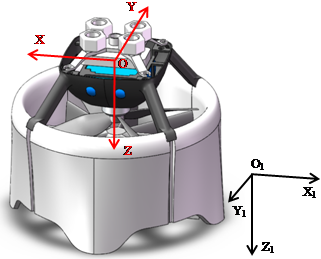
\includegraphics[width=0.6\textwidth]{figure/body1.png}
    \caption{\label{fig:body}机体结构}
\end{figure}
\subsection{机电控制系统}
机电控制系统是是无人机的“大脑”和“神经中枢”，负责感知自身状态、处理信息并精确控制各个执行机构。其主要包括微控制器，传感器和执行器。接下来将对该无人机附带的机电控制系统的各个模块进行逐一介绍。

\begin{itemize}
    \item 微控制器，本文使用的为控制为意法半导体公司的STM32系列的STM32F767芯片，基于ARM架构的Cortex-M7内核设计。最高主频可达 216MHz。集成单精度浮点运算单元（FPU）和DSP指令集，能够轻松胜任飞行控制环节中的自身状态感知算法和闭环控制算法。此外，集成了PWM、IIC、SPI、UART等常用通信接口，能够与其它硬件模块实现低时延高可靠的通信。同时，片内集成2MB的的Flash存储器与 512KB 的SRAM存储器，能够提供充足空间来执行内存占用较大的高阶卡尔曼滤波等算法。
    \item 惯性测量单元（IMU），惯性测量单元能够高频率地采集无人机的角速度和加速度，为飞控计算机提供解算飞行状态所需的原始数据，是无人机的“小脑”。本文使用的惯性测量单元是InvenSense公司的ICM-20602。该芯片量程范围大，支持±2000dps陀螺量程、±16g加速度量程。且测量噪声小，速率噪声典型值为0.004 °/s/√Hz，加速度计噪声典型值为 100 µg/√Hz，该芯片最高采样频率为1kHz。配合上卡尔曼滤波算法能够实现高精度的位姿估计。
    \item 磁力计，磁力计用于感知地磁北的方向，在小范围运动的情况下，该方向可以认为与地球北极的方向成一个固定的夹角。本文使用的磁力计是iSentek的IST8310三轴霍尔效应磁传感器。该传感器的测量范围大，支持三轴±1600µT磁感应强度，该量程足以测量地磁场的方向和大小。最高采样频率为200Hz。磁力计的数据能够保证位姿估计时，航向角的估计不会发散。
    \item 激光测距模块，激光测距模块被安装在飞机的底部，是无人机领域用于感知离地高度的常用传感器。本文使用的激光测距模块是意法半导体公司的VL53l1X激光测距传感器。测量精度为±5\%，采样频率为50Hz。读取测量数据能够感知离地高度进而能够对地面效应带来的扰动做抗扰控制。
    \item 电池，本文使用的电池是容量为1680mAh的4S1P的航模电池，电池的输出电压为16.8V，最大持续输出电流为20A。
    \begin{figure}
        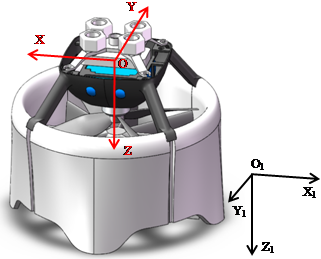
\includegraphics[width=0.6\textwidth]{figure/body1.png}
        \caption{航模电池}
    \end{figure}
    \item 电机电调系统，电机电调系统用于带动主螺旋桨的转动。本文使用的电机是翼飞的2806.5无刷直流电机，其KV值为1300KV，定子直径28mm，高度6.5mm。使用的电调的通信方式为PWM通信，控制频率为200Hz。其额定电压为16V，额定电流为30A。
    \begin{figure}
        \centering
        \begin{minipage}[b]{0.45\textwidth}
            \centering
            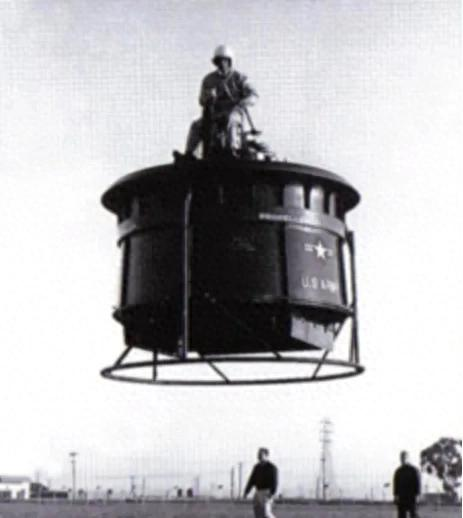
\includegraphics[height=0.22\textheight]{figure/Hiller VZ-1.jpeg}
        \end{minipage}
        \hfill  % 产生弹性水平间距
        \begin{minipage}[b]{0.45\textwidth}
            \centering
            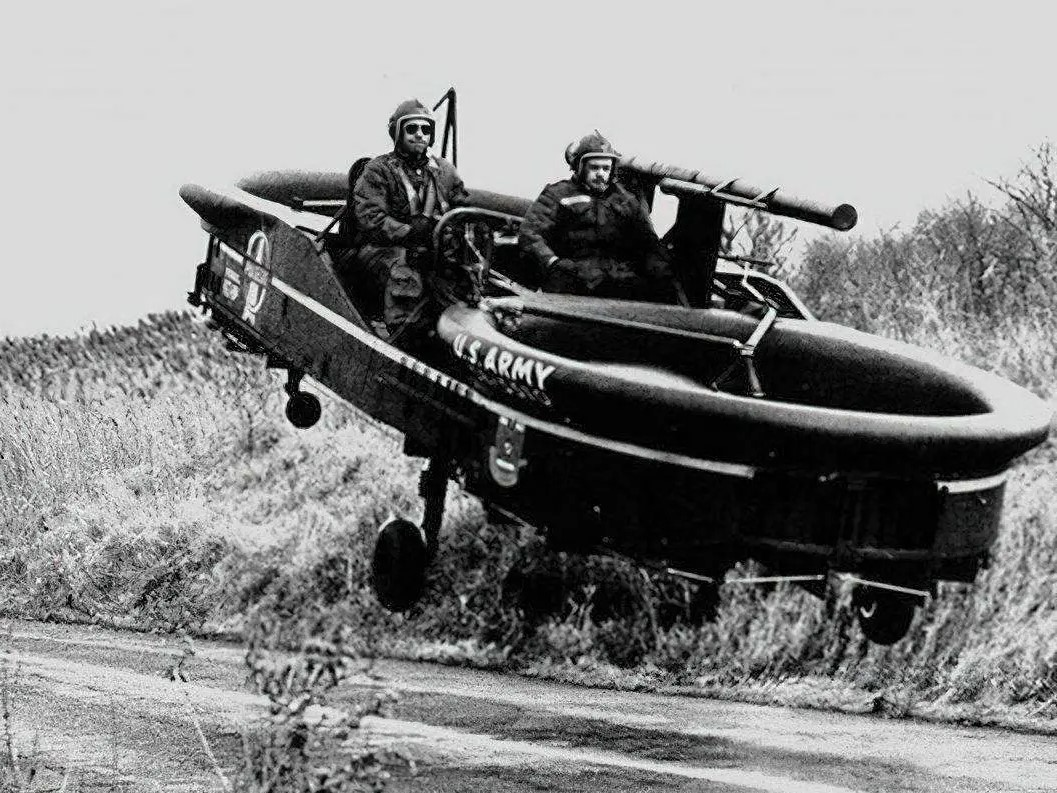
\includegraphics[height=0.22\textheight]{figure/Piasecki VZ-8.jpg}
        \end{minipage}
        \caption{电机电调系统}
    \end{figure}
    \item 舵机，舵机用于控制螺旋桨下方的控制舵面的转动，是无人机实现姿态闭环控制的关键。本文使用的舵机是银燕的ES9251舵机，该舵机为塑料齿轮舵机，单个舵机重量仅为2.8g，最大输出力矩为0.02646N·m。舵机的通信方式为PWM通信，最高控制频率为50Hz。
    \begin{figure}
        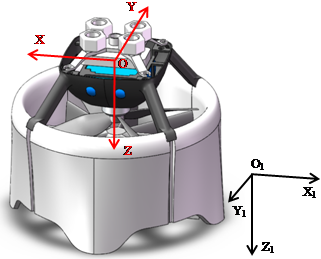
\includegraphics[width=0.6\textwidth]{figure/body1.png}
        \caption{舵机}
    \end{figure}
    \item 电路板，为了将整个电子系统的各个模块连接起来，设计了两块电路板，分别是飞行控制板和舵机驱动板。这两块电路板上各搭载了一块微控制器芯片。电路板将其中搭载的芯片和电子模块通过印制电路连接，并将微传感器的各个物理通信口，通过线对板针座引出。飞行控制板用于执行复杂的位姿估计算法，闭环控制算法，而舵机控制板主要执行指令控制舵机以及获取传感器输出。为了能够测出无人机质心的角速度和加速度，IMU被设计放置在更靠近质心的飞行控制板。而为了使磁力计尽量少地受到无刷电机的磁场干扰，它被设计放置在远离无刷电机的舵机驱动板。此外，激光测距传感器也需要放置在底部的舵机驱动板上，用于测量下方离地高度。
    \begin{figure}
        \centering
        \begin{minipage}[b]{0.45\textwidth}
            \centering
            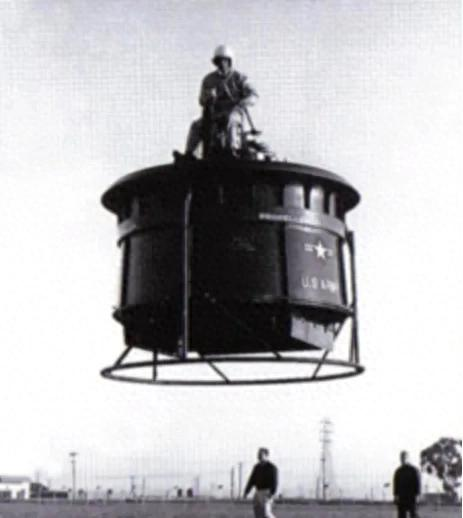
\includegraphics[height=0.22\textheight]{figure/Hiller VZ-1.jpeg}
            \caption{飞行控制板}
        \end{minipage}
        \hfill  % 产生弹性水平间距
        \begin{minipage}[b]{0.45\textwidth}
            \centering
            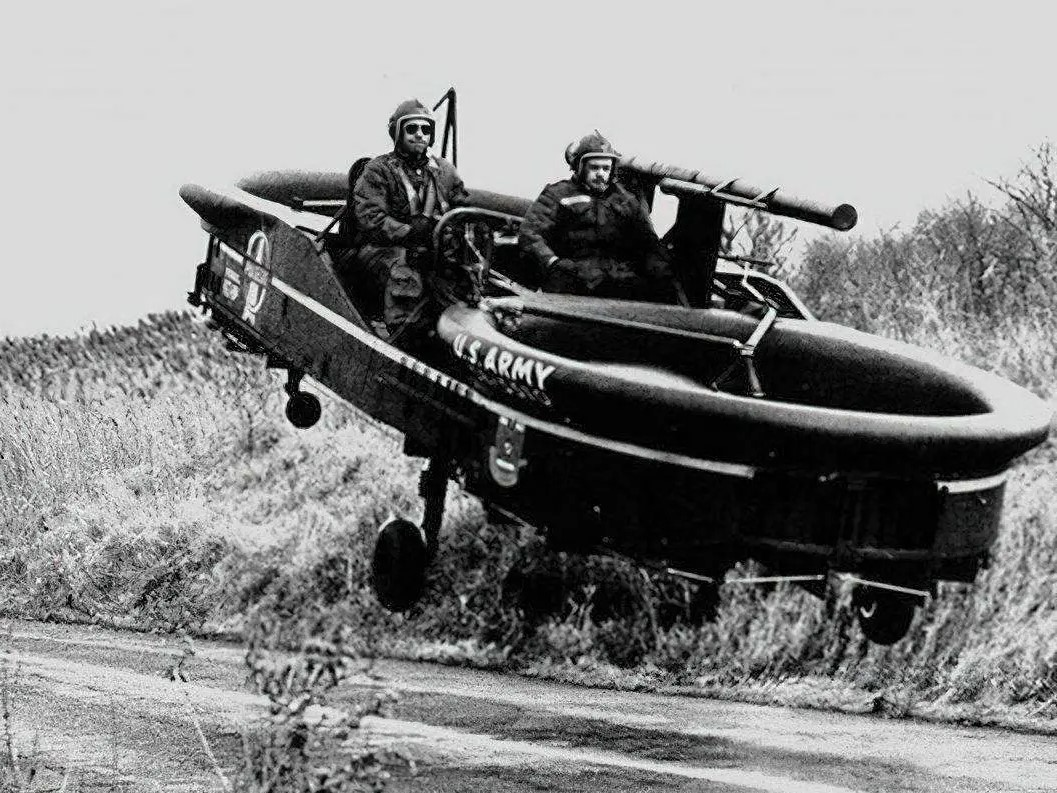
\includegraphics[height=0.22\textheight]{figure/Piasecki VZ-8.jpg}
            \caption{舵机驱动板}
        \end{minipage}
    \end{figure}
  \end{itemize}

\subsection{程序设计}
微控制器的程序是基于C++语言设计的，并且部署FreeRTOS实时操作系统进行任务管理。程序主要负责以下内容：遥控器控制指令获取，传感器数据读取，传感器数据预处理，无人机位姿估计，闭环控制器算法处理，输出执行器指令等。
具体程序设计如图\ref{fig:software_figure}所示。
\begin{figure}
    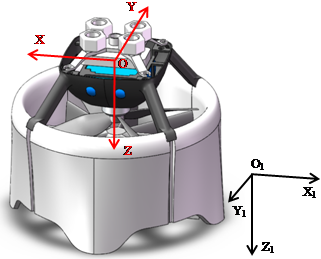
\includegraphics[width=0.6\textwidth]{figure/body1.png}
    \caption{\label{fig:software_figure}程序设计框图}
\end{figure}

\section{坐标系的定义}
清晰、准确地定义无人机坐标系是至关重要的基础性工作，是确保论文科学性和严谨性的前提。接下来将逐一介绍本文使用的坐标系以及相关符号的定义。

\subsection{地面坐标系}
地面坐标系是右手系，满足右手定则。取无人机的起飞点作为地面坐标系的原点\( O_e \)，定义坐标轴\( O_e - X_e \)过原点\( O_e \)向地理北向（North），坐标轴\( O_e - Y_e \)过原点\( O_e \)向地理东向（East），由右手定则，坐标轴\( O_e - Z_e \) 竖直向下（Down）。根据定义可知，该地面坐标系\( O_e - X_e Y_e Z_e \)和地面相对静止，因此，地面坐标系为惯性系。地面坐标系文中也称为地面系。

\subsection{机体坐标系}
机体坐标系也是右手系，同样满足右手定则。取无人机的质心为机体坐标系的原点\( O_b \)，定义坐标轴\( O_b - X_b \)过原点\( O_b \)指向无人机的正前方，定义坐标轴\( O_b - Y_b \)过原点\( O_b \)指向无人机的正右方，由右手定则，坐标轴\( O_e - Z_e \) 过原点\( O_b \)指向无人机的正下方。类似的，机体坐标系和无人机相对静止，机体坐标系为非惯性系。机体坐标系文中也称为机体系。

\begin{figure}
    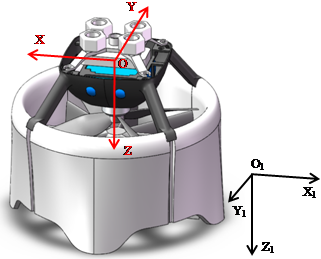
\includegraphics[width=0.6\textwidth]{figure/body1.png}
    \caption{\label{fig:cordinate}地面坐标系和机体坐标系}
\end{figure}

地面坐标系和机体坐标系的关系如图\ref{fig:cordinate}所示。值得注意的是，在三维空间中，同一个矢量，在两个坐标系下的投影是不一样的。为了防止表述上出现歧义，此处定义，三维空间中的矢量在地面坐标系下的投影记为$(·)^e$，在机体坐标系下的投影记为$(·)^b$。

\subsection{坐标系之间的旋转关系}
坐标系之间的旋转关系是进行姿态控制、导航和传感器融合的基础。常用的表示方法主要有四种：欧拉角、旋转矩阵、四元数和轴角法。在现有的飞控程序中，最常用的是欧拉角和四元数。欧拉角是较为直观的表示方式，但是其存在万向锁（gimbal lock）的问题\cite{quan2018}，当俯仰角为±90°时，会出现自由度退化的问题。由于本文设计的无人机控制的俯仰角不会超过±45°，因此，不需要考虑万向锁的情况。

（1）欧拉角

欧拉角是描述刚体在三维空间中旋转关系的一种常用方法，它通过三次绕指定坐标轴的旋转，将地面坐标系变换到机体坐标系。本文使用的欧拉角是“ZYX欧拉角”，即旋转顺序为：首先绕地面坐标系的 $O_e - Z_e$ 轴旋转角度 $\psi$（偏航角，yaw），然后绕新坐标系（第一次旋转后）的 $O_e ' - Y_e '$ 轴旋转角度 $\theta$（俯仰角，pitch），最后绕最新坐标系（第二次旋转后）的 $O_e '' - X_e ''$ 轴旋转角度 $\varphi$（滚转角，roll）。这种旋转方式也称为内旋（intrinsic rotation），即每次旋转绕当前坐标系的轴进行。
规定$(\psi, \theta, \varphi)$的角度范围为：
\begin{equation}
\psi \in (-\pi,\ \pi], \quad \theta \in \left[-\frac{\pi}{2},\ \frac{\pi}{2}\right], \quad \varphi \in (-\pi,\ \pi].
\end{equation}
\begin{figure}
    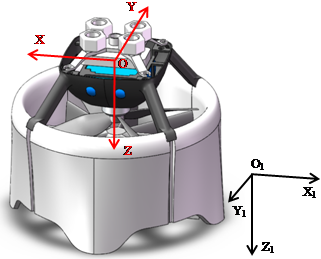
\includegraphics[width=0.6\textwidth]{figure/body1.png}
    \caption{\label{fig:eular_angle}“ZYX欧拉角”的定义}
\end{figure}

（2）旋转矩阵

定义从机体坐标系到地面坐标系的旋转矩阵 $\bm{R}_{b}^{e}$，使得对三维空间中的任意矢量$\bm{v}$ 在机体坐标系中的投影$\bm{v}^b$ 以及其在地面坐标系中的投影 $\bm{v}^e$ 满足：
\begin{equation}
\bm{v}^e = \bm{R}_{b}^{e} \, \bm{v}^b.
\end{equation}
根据旋转矩阵的特性，从地面坐标系到机体坐标系的旋转矩阵$\bm{R}_{e}^{b} = \bm{R}_{b}^{eT}$ ，且满足：
\begin{equation}
\bm{v}^b = \bm{R}_{e}^{b} \, \bm{v}^e.
\end{equation}
按照上述顺序，旋转矩阵可通过依次左乘每次旋转对应的基本旋转矩阵得到。绕X、Y、Z轴旋转的基本旋转矩阵的定义分别如下：
\begin{equation}
\bm{R}_x(\varphi) = \begin{bmatrix}
1 & 0 & 0 \\
0 & \cos\varphi & -\sin\varphi \\
0 & \sin\varphi & \cos\varphi
\end{bmatrix},
\bm{R}_y(\theta) = \begin{bmatrix}
\cos\theta & 0 & \sin\theta \\
0 & 1 & 0 \\
-\sin\theta & 0 & \cos\theta
\end{bmatrix},
\bm{R}_z(\psi) = \begin{bmatrix}
\cos\psi & -\sin\psi & 0 \\
\sin\psi & \cos\psi & 0 \\
0 & 0 & 1
\end{bmatrix}.
\label{eq:single_eular_R}
\end{equation}

对于ZYX内旋顺序，旋转矩阵 $\bm{R}_{e}^{b}$ 的计算过程为：
1. 第一次旋转绕地面系 $O_e - Z_e$ 轴旋转 $\psi$，得到坐标系 $\{1\}$，有 $\bm{R}_{e}^{1} = \bm{R}_z(\psi)$。
2. 第二次旋转绕坐标系 $\{1\}$ 的 $O_e' - Y_e'$ 轴旋转 $\theta$，得到坐标系 $\{2\}$。由于旋转在当前坐标系中进行，且当前坐标系的基仍为标准正交基，该旋转在坐标系 $\{1\}$ 中的表示即为 $\bm{R}_y(\theta)$。因此从世界到坐标系 $\{2\}$ 的旋转矩阵为 $\bm{R}_{e}^{2} = \bm{R}_y(\theta) \bm{R}_z(\psi)$。
3. 第三次旋转绕坐标系 $\{2\}$ 的 $O_e'' - X_e''$ 轴旋转 $\varphi$，类似地得到从世界到物体坐标系的旋转矩阵：
\begin{equation}
\bm{R}_{e}^{b} = \bm{R}_x(\varphi) \bm{R}_y(\theta) \bm{R}_z(\psi).
\end{equation}
展开后得从地面坐标系到机体坐标系的旋转矩阵$\bm{R}_{e}^{b}$：
\begin{equation}
\bm{R}_{e}^{b} = 
\begin{bmatrix}
\cos\theta\cos\psi & \cos\theta\sin\psi & -\sin\theta \\
\sin\varphi\sin\theta\cos\psi - \cos\varphi\sin\psi & \sin\varphi\sin\theta\sin\psi + \cos\varphi\cos\psi & \sin\varphi\cos\theta \\
\cos\varphi\sin\theta\cos\psi + \sin\varphi\sin\psi & \cos\varphi\sin\theta\sin\psi - \sin\varphi\cos\psi & \cos\varphi\cos\theta
\end{bmatrix}.
\end{equation}

\section{运动学模型}
运动学建模是指在不考虑引起运动的力（如重力、惯性力、摩擦力等）的情况下，使用数学工具对物体或机构（特别是连杆机构）的运动属性（如位置、速度、加速度）进行描述、分析和计算的过程。本小节将针对涵道式无人机的机身进行运动学分析，用数学语言建立其位置姿态与时间之间的关系。

记无人机在地面系下的位置矢量为$\bm{P}$，无人机在地面系下的速度矢量为$\bm{v}$，记无人机的欧拉角为$\bm{\eta}=[\varphi \quad \theta \quad \psi]^T$，记无人机的角速度矢量为$\bm{\omega}$，那么$\bm{\omega}$在机体系下的投影为$\bm{\omega}^b = [p \quad q \quad r]^T$。
可得速度和位置之间的关系为：
\begin{equation}
    \dot{\bm{P}}^e = \bm{v}^e
    \label{eq:d_pos}
\end{equation}

而无人机的角速度和与其欧拉角的关系可参考Ducard等人\cite{Ducard2009Flight}的推导结果，此处直接引述其结论:

\begin{equation}
\bm{\omega}^b = \dot{\psi} \bm{R}_\varphi \bm{R}_\theta \bm{e}_3 + \dot{\theta} \bm{R}_\varphi \bm{e}_2 + \dot{\varphi} \bm{e}_1
\label{eq:eular_rate}
\end{equation}
其中，
\begin{equation}
\bm{e}_1 = 
\begin{bmatrix}
1 \\
0 \\
0
\end{bmatrix}, \quad \bm{e}_2 = 
\begin{bmatrix}
0 \\
1 \\
0
\end{bmatrix}, \quad \bm{e}_3 = 
\begin{bmatrix}
0 \\
0 \\
1
\end{bmatrix}.
\label{eq:unit_vector}
\end{equation}
由式\eqref{eq:single_eular_R}，\eqref{eq:eular_rate}，\eqref{eq:unit_vector}，可得：
\begin{equation}
\dot{\bm{\eta}} = 
\begin{bmatrix}
1 & \sin\varphi\tan\theta & \cos\varphi\tan\theta \\
0 & \cos\varphi & -\sin\varphi \\
0 & \sin\varphi & \cos\varphi
\end{bmatrix}
\bm{\omega}^b
\end{equation}
为了简化表述，令矩阵$\bm{Q}$为：
\begin{equation}
\bm{Q} = 
\begin{bmatrix}
1 & \sin\varphi\tan\theta & \cos\varphi\tan\theta \\
0 & \cos\varphi & -\sin\varphi \\
0 & \sin\varphi & \cos\varphi
\end{bmatrix}
\end{equation}
最终，能够得到无人机的角速度和姿态角的变化率之间的关系为：
\begin{equation}
    \dot{\bm{\eta}} = \bm{Q}\bm{\omega}^b
    \label{eq:d_eular}
\end{equation}

\section{动力学模型}
动力学建模是指在考虑引起运动的根本原因——力与力矩的前提下，运用物理学基本定律建立数学模型。在动力学建模领域，牛顿-欧拉方法是一种广泛应用于多体系统动力学建模的递推算法，它基于经典力学中的牛顿第二定律（描述刚体平动）和欧拉方程（描述刚体转动），通过正向和反向递推，系统地建立机器人等机构各连杆之间的运动学关系。和大多数无人机领域的学术研究一样，本文假设涵道式无人机的各个零件认为是质量均匀分布的刚体模型。

由前文对机体结构的介绍可知，涵道式无人机可以看作六个相互独立的刚体，分别是无人机的机身、螺旋桨以及四个控制舵面。由单个控制舵面的质量仅为3.2g，控制舵面的活动范围较小，为避免动力学模型过于复杂，本文作出必要的简化，认为控制舵面是能够产生气动力而质量为零的刚体，而将控制舵面的质量计入机身质量。

\begin{figure}
    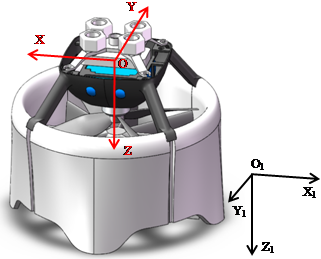
\includegraphics[width=0.6\textwidth]{figure/body1.png}
    \caption{涵道式无人机的各个刚体零件}
\end{figure}

无人机的位置动力学可由牛顿第二定律推导出。记无人机受到的除重力之外的合外力为$\bm{F}$，无人机质量为$m$，当地重力加速度大小为$g$，无人机的加速度为$\bm{a}$，由牛顿第二定律可以得到，在地面坐标系下的加速度$\bm{a}^e$为：
\begin{equation}
    \bm{a}^e = \dot{\bm{V}}^e = g\bm{e}_{3} + \bm{F}^e m^{-1}
\end{equation}
整理可得：
\begin{equation}
    \dot{\bm{V}}^e = g\bm{e}_{3} + \bm{R}_b^e\bm{F}^b m^{-1}
    \label{eq:d_vel}
\end{equation}

无人机的姿态动力学可由欧拉方程推导出。记无人机受到的合外力矩为$\bm{M}$，无人机的角动量为$\bm{L}$，无人机在机体系下的转动惯量矩阵为$\bm{J}$。
显然，机体系下的转动惯量矩阵$\bm{J}$是一个常矩阵，且由该无人机结构\ref{fig:body}可以看出，其质量分布关于平面$X_b O_b Z_b$和平面$Y_b O_b Z_b$对称分布，机体坐标系的三个轴均为刚体的惯性主轴，因此，矩阵$\bm{J}$为对角阵\cite{quan2018}。记$J_x$、$J_y$和$J_z$分别为机体对三轴的主转动惯量，得：
\begin{equation}
    \bm{J} = 
    \begin{bmatrix}
        J_x & 0 & 0 \\
        0 & J_y & 0 \\
        0 & 0 & J_z
    \end{bmatrix}
\end{equation}
由欧拉方程，无人机受到的合外力矩在机体坐标系下的投影$\bm{M}^b$可直接给出：
\begin{equation}
    \bm{M}^b = \bm{J}\cdot\dot{\bm{\omega}^b}+\bm{\omega}^b\times(\bm{J}\cdot\bm{\omega}^b)
\end{equation}
经整理，可得：
\begin{equation}
    \dot{\bm{\omega}^b} = \bm{J}^{-1}(\bm{M}^b - \bm{\omega}^b\times(\bm{J}\cdot\bm{\omega}^b))
    \label{eq:d_omega}
\end{equation}

至此，无人机的基本运动学和动力学模型可以通过\eqref{eq:d_pos}、\eqref{eq:d_eular}、\eqref{eq:d_vel}、\eqref{eq:d_omega}给出，整理可得：
\begin{equation}
    \begin{cases} 
        \dot{\bm{P}}^e = \bm{v}^e \\ 
        \dot{\bm{V}}^e = g\bm{e}_{3} + \bm{R}_b^e\bm{F}^b m^{-1} \\ 
        \dot{\bm{\eta}} = \bm{Q}\bm{\omega}^b \\ 
        \dot{\bm{\omega}^b} = \bm{J}^{-1}(\bm{M}^b - \bm{\omega}^b\times(\bm{J}\cdot\bm{\omega}^b)) 
    \end{cases} 
\end{equation}

值得注意的是，上文的动力学模型中，存在两个未知量$\bm{F}$和$\bm{M}$，即无人机受到的除重力以外的合外力和合外力矩。这部分作用力和作用力矩是涵道式无人机的受力分析中最复杂的，也是涵道式无人机所独有的。接下来将展开分析这些力和力矩，以完善整个动力学模型。

\section{涵道式无人机受到的力和力矩}
由于涵道式无人机独特的机体结构，其飞行状态下的气动特性相比于多旋翼无人机更为复杂。涵道式无人机在飞行过程中所受到作用，主要包括机身、螺旋桨、控制舵面以及反扭矩襟翼带来的力和力矩。接下来，将根据现有主流理论，使用机理法对机体受到的各个力和力矩进行逐一分解。

\subsection{涵道风扇动力学}
涵道风扇是指外层由涵道壁包裹的经特殊设计的螺旋桨。在涵道风扇的稳定工作状态下，空气从上方涵道口被吸入，经过涵道和涵道风扇的共同作用下，被加速加压，并且从下方涵道口被排出。这个过程由于存在涵道壁对气流的约束和压缩作用，使得涵道风扇相比于孤立旋翼有更高的气动效率。

稳定工作状态下涵道风扇产生的力和力矩，与多种因素存在复杂耦合关系，包括螺旋桨转速、桨盘面积、涵道无人机的迎角、气流速度、无人机飞行速度等因素。对此，目前数值法分析是学术界的主流研究方法。Ohanian经过大量试验并通过数值法深入研究后，使用轴向的拉力和垂直于轴向的侧向力的模型来解释涵道风扇产生的总作用力，并得出拉力$T_{fan}$和侧向力$N_{fan}$可由下面式子给出\cite{2012Nondimensional}：
\begin{equation}
    \begin{cases}
        T_{fan} = \frac{1}{2}\rho \pi C_T R^4 \Omega^2 \\
        N_{fan} = \frac{1}{2}\rho \pi C_N R^4 \Omega^2 
    \end{cases}.
\end{equation}
其中，$C_T$和$C_N$都是无量纲系数，分别是涵道风扇的拉力系数和侧向力系数，且它们满足下面式子\cite{2012Nondimensional}：
\begin{equation}
    \begin{cases}
        C_T = C_{T0} + (J - J_0) (C_{T_{J0}} + C_{T_J} cos\alpha_{df}) \\
        C_N =  (J - J_0) C_{N_J} sin\alpha_{df}
    \end{cases}.
\end{equation}

和开放旋翼类似，涵道风扇的作用力和作用力矩的计算同样通过拉力系数和扭矩系数计算出。根据现有学者的研究\cite{LUO2024263}，涵道风扇产生的气动拉力$T_p$以及风扇扭矩$M_{fan}$可由下面式子给出：
\begin{equation}
    \begin{cases} 
        T_p = \rho S \Omega^2 R^2 C_p \\
        M_{fan} = \rho S \Omega^2 R^3 C_q
    \end{cases} 
\end{equation}
其中，$\Omega$是螺旋桨的转速，$R$是螺旋桨桨尖半径，$C_p$和$C_q$分别是是螺旋桨拉力系数和扭矩系数。值得注意的是，这些气动系数与气流环境，飞行状态深度耦合，学术界暂时未出现统一且研究充分的理论，本文不作展开论述。不少学者针对该现象，通过数值方法开展深度研究，尝试解释该特性\cite{cheng2021, han2022}。



现阶段涵道风扇动力学的主流分析模型是基于动量理论与叶素理论。



在涵道风扇处于稳定工作状态时，由于涵道壁的约束作用，气体流动状态处于轴流状态，即来流方向与涵道风扇的旋转轴线平行或重合，流经涵道风扇的气流是轴对称的。在该状态下可以通过动量理论分析螺旋桨的推力大小。

经典的Rankine-Froude动量理论将涵道风扇简化为一个均匀的激励盘，气流通过盘面时压力发生突变，动量瞬间增加。通过该简化模型，对空气来流使用动量定理，从而近似的计算出推力大小。

假设流动是定常、不可压、无粘且无旋的，并认为涵道入口前方的来流是均匀的。设气流在无穷远处的速度大小为$V_0$，气流在接触到螺旋桨前的速度为$V_1$，气流在接触到螺旋桨后，速度骤升为$V_2$，

扩张比${\sigma}_d$是一个至关重要的几何参数。它指的是涵道下方出风口横截面面积$S'$与桨盘面积$S$之比，直接决定了气流在涵道内部的减速增压过程，对于一个结构固定的涵道风扇而言，该扩展比${\sigma}_d$是常量。



\begin{figure}
    \centering
    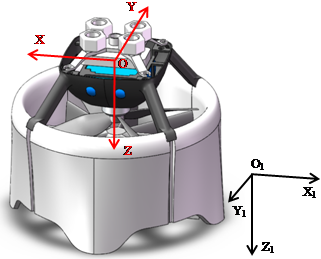
\includegraphics[width=0.6\textwidth]{figure/body1.png}
    \caption{轴流状态的气动分析}
\end{figure}

陀螺力矩

\subsection{涵道壁动力学}

\subsection{控制舵面动力学}

\subsection{反扭距襟翼动力学}

\section{实验样机}

\section{本章小结}